% \begin{figure}[t]
    \centering
    \begin{tikzpicture}[remember picture, overlay, yshift=-3cm]
        %% Horizontal bar
        \draw[very thick] (3,0) -- (-3,0);
        % FPT
        \draw (-2,0) parabola bend (0,2) (2,0);
        \node at (0,1) {\FPT};
        % W[1]
        \draw (-2.5,0) parabola bend (0,3) (2.5,0);
        \node at (0,2.5) {\textsf{W}[1]};
        % XP
        \draw[rounded corners] (-3,0) .. controls (-1,4) and (5,9) .. (3,0);
        \node at (2, 4) {\XP};
        % para-NP
        \draw[rounded corners] (3,0) .. controls (1,4) and (-5,9) .. (-3,0);
        \node at (-2, 4) {\pNP};
    \end{tikzpicture}
    % \caption
    % [Relations among the parameterized complexity classes]
    % {
    %     Relations among the parameterized complexity classes.
    %     Inspired by the depiction from Flum and Grohe \cite[p.~97]{Flum2006}.
    % }
    % \label{fig:complexityClasses}
% \end{figure}
